\documentclass[tikz]{standalone}

\usepackage{tikz}
\usetikzlibrary{positioning}

\begin{document}

\tikzset{%
	every neuron/.style={
		circle,
		draw,
		minimum size=1cm
	},
	neuron missing/.style={
		draw=none, 
		scale=2,
		text height=0.3cm,
		execute at begin node=\color{black}$\vdots$
	},
}

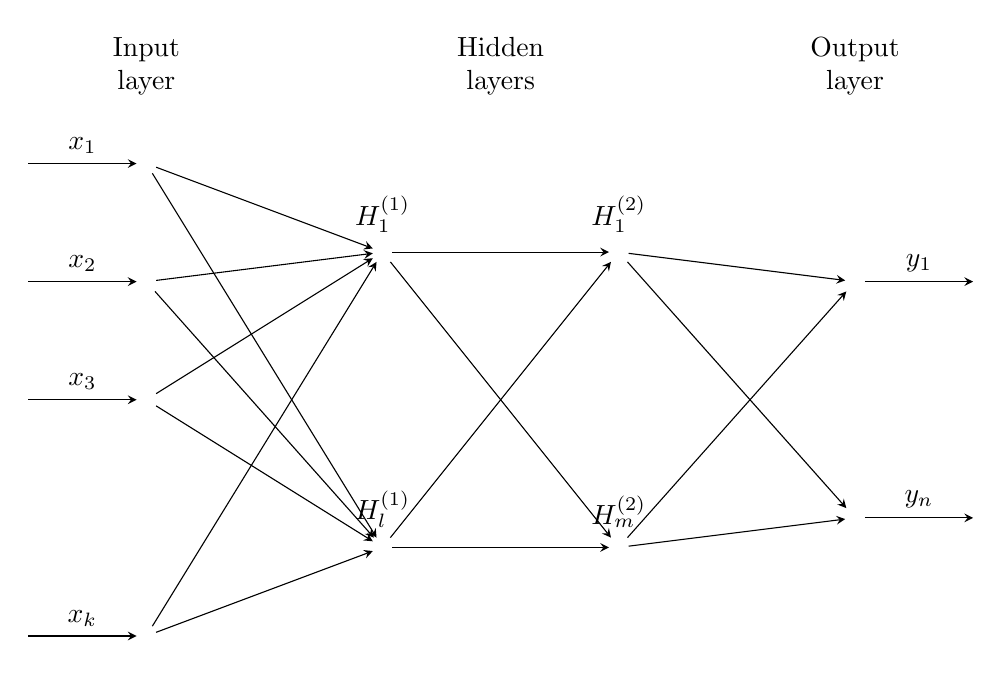
\begin{tikzpicture}[x=1.5cm, y=1.5cm, >=stealth]

\foreach \m/\l [count=\y] in {1,2,3,missing,4}
	\node [every neuron/.try, neuron \m/.try] (input-\m) at (0,2.5-\y) {};

\foreach \m [count=\y] in {1,missing,2}
	\node [every neuron/.try, neuron \m/.try ] (hidden1-\m) at (2,2-\y*1.25) {};

\foreach \m [count=\y] in {1,missing,2}
	\node [every neuron/.try, neuron \m/.try ] (hidden2-\m) at (4,2-\y*1.25) {};

\foreach \m [count=\y] in {1,missing,2}
	\node [every neuron/.try, neuron \m/.try ] (output-\m) at (6,1.5-\y) {};

\foreach \l [count=\i] in {1,2,3,k}
	\draw [<-] (input-\i) -- ++(-1,0)
		node [above, midway] {$x_\l$};

\foreach \l [count=\i] in {1,l}
	\node [above] at (hidden1-\i.north) {$H^{(1)}_\l$};

\foreach \l [count=\i] in {1,m}
	\node [above] at (hidden2-\i.north) {$H^{(2)}_\l$};

\foreach \l [count=\i] in {1,n}
	\draw [->] (output-\i) -- ++(1,0)
		node [above, midway] {$y_\l$};

\foreach \i in {1,...,4}
	\foreach \j in {1,...,2}
		\draw [->] (input-\i) -- (hidden1-\j);

\foreach \i in {1,...,2}
	\foreach \j in {1,...,2}
		\draw [->] (hidden1-\i) -- (hidden2-\j);

\foreach \i in {1,...,2}
	\foreach \j in {1,...,2}
		\draw [->] (hidden2-\i) -- (output-\j);

%\foreach \l [count=\x from 0] in {Input, Hidden, Hidden, Ouput}
\node [align=center, above] at (0,2) {Input \\ layer};
\node [align=center, above] at (3,2) {Hidden \\ layers};
\node [align=center, above] at (6,2) {Output \\ layer};

\end{tikzpicture}

\end{document}
